\documentclass{beamer}

\usepackage{beamer_tom}
\graphicspath{{./images/}}

\institute{INRIA Saclay}
\author{Thomas Moreau}
\title{
    Extraction of Nystagmus Patterns from Eye-Tracker Data\\
    with Convolutional Sparse Coding.
}

\setbeamertemplate{title page}[frame]
\def\extraLogo{}

\begin{document}

    \begin{frame}
        \titlepage
    %	\biblio{}
    \end{frame}

    \frame{
        \frametitle{Pathological Infantile Nystagmus}

        \begin{columns}[c]
            \column{.5\textwidth}
            \begin{itemize}
                \item Sporadic movement of the eye.
                \item Link to several conditions:\\Gliomas, albinism, down syndrom, ...
                \item Classification of 16 different Waveforms [Dell'Osso et al. 75]
            \end{itemize}
            \column{.5\textwidth}
            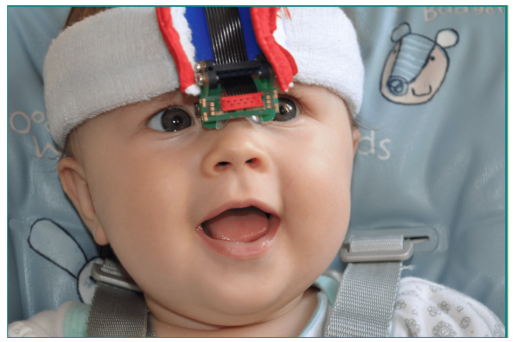
\includegraphics[width=\textwidth]{eyefant.png}
            \keypoint{Recording the nystagmus with an eye tracker}
        \end{columns}

        \vskip2em
        Can extract the waveform automatically?
        \strongpoint{Use Convolutional Dictionary Learning!}
    }

    \frame[t]{
        \frametitle{Eyetracker recording}
        \vskip2em
        {\centering\alt<2->{
            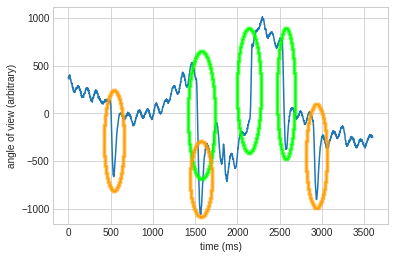
\includegraphics[width=.7\textwidth]{angle_of_view_highlighted}\\[.5em]
            \begin{itemize}
                \item Eye blinks artifacts
                \item Super imposed gaze movement: low freq + saccades.
            \end{itemize}
        }{
            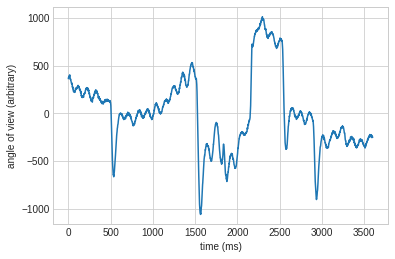
\includegraphics[width=.7\textwidth]{angle_of_view}\\[.5em]
        }}
    }

    \frame{
        \frametitle{Joint detrending and CDL}

        Ad hoc detrending tends to alter the waveform
        \begin{itemize}
            \item Filtering \keypoint{break harmonics}
            \item TV-L1 \keypoint{hard to chose the reg. parameter}
        \end{itemize}

        \vskip2em
        Idea, joint detrending with CDL:
        \[
            \argmin_{z, D, y} \frac12\|x - z*D - y\|_2^2
                + \lambda \|z\|_1 + \lambda_{TV}\|\nabla y\|_1
        \]
        \begin{itemize}
            \item Does not complexify the optimization (bi-convex)
            \item Equivalent to iterative application of a detrending method
            \item Both components will be co-adapted
        \end{itemize}

    }

    \frame{
        \frametitle{Results}

        \begin{columns}[T]
            \column{.5\textwidth}
            Pattern recovery on simulated data\\[1em]
            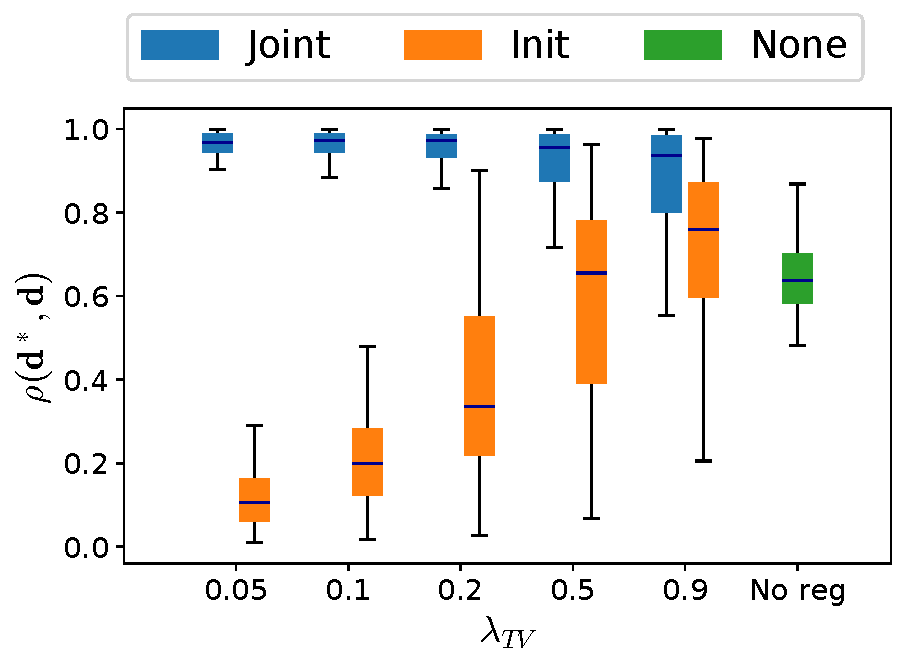
\includegraphics[width=\textwidth]{pearson_reg=0,5.pdf}
            \column{.5\textwidth}
            Qualitative results on real signals\\[1em]
            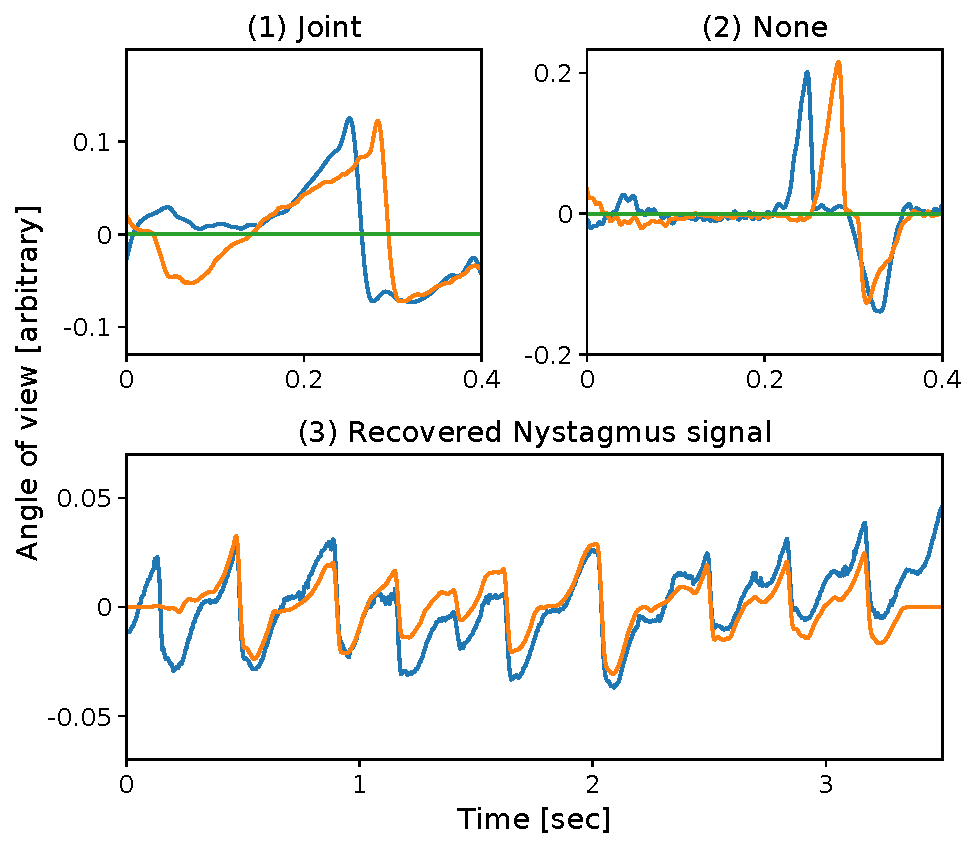
\includegraphics[width=\textwidth]{pattern_trend_2.pdf}
        \end{columns}
    }


\end{document}
